% !TeX spellcheck = nl_NL
\documentclass{article}
\usepackage{hyperref}
\usepackage{graphicx}
\usepackage{listings}
\title{Project ComputerSystemen}
\author{Arno De Witte (500504) \\Wout Van Riel (500229)  \\Email: \href{mailto:Arno.De.Witte@vub.ac.be}{Arno.De.Witte@vub.ac.be} \\ \href{mailto:Wout.Van.Riel@vub.ac.be}{Wout.Van.Riel@vub.ac.be} \\ 
Vrije Universiteit Brussel}
\date{6 januari 2014}
\begin{document}
\maketitle
\newpage
\tableofcontents
\newpage


\section{Voorwoord}
Dit spel is gemaakt als project voor het vak Computersystemen.
Het project had als opdracht een spel te maken of een decoder voor een bepaalde encodering.
Het spel had meteen de aandacht en we begonnen na te denken over welke klassieker we zouden maken tijdens ons project.
Aangezien onze kennis van (masm) assembly niet al te groot was bij aanvang van het project, beseften we dat het spel in een 2D-omgeving gespeeld zou worden.
Space-invader was aanlokkelijk, maar niet origineel dus kregen we het idee om een avatar tegenkomende obstakels te laten ontwijken en de dit object de kans te geven om deze obstakels uit te schakelen door op hen te schieten.
We hadden al eerder spellen gezien met een gelijkaardig thema en het trok ons wel aan. Dus maakten we het spel Asteroid Field.

\section{Het spel}\label{spel}

Het concept van het spel is eenvoudig: probeer niet geraakt te worden door de asteroiden die naar de ruimtesonde komen.
Een asteroide wordt nooit op dezelfde plaats gecreëerd waardoor het spel telkens een andere ervaring is.
Om het niet eentonig en simpel te houden, zijn er levels ge\"implementeerd die na een bepaalde tijd verhogen.
Dus hoe langer de ruimtesonde kan overleven in het asteroideveld, hoe moeilijker de levels worden.
De score staat los van de levels, maar is wel aan een ander, minder logisch, aspect van het spel gekoppeld.
Elk punt dat je scoort is goed voor \'e\'en kogel dat je kan afvuren.
Wanneer de score op nul staat, is het enigste wat je kan doen de asteroiden vingervlug ontwijken en hopen dat je toch toevallig een asteroide hebt geraakt met een verdwaalde kogel.
Voor elke asteroide dat geraakt kan worden met een kogel, worden er drie punten bij de totaalscore geteld en voor elke kogel dat afgevuurd wordt, trekt het spel \'e\'en punt van de totaalscore af.
Wie een hoge score wil, kan dus beter al zijn kogels goed gebruiken.
Wanneer je geraakt wordt, zal het scherm rood flitsen.

\section{Besturing}

Het spel heeft maar drie toetsen nodig om gespeeld te worden. Namelijk de drie pijltjes: omhoog, omlaag en rechts.
Om het schip omhoog te laten gaan, moet de omhoogpijl van het toetsenbord ingedrukt worden.
Om een kogel af te vuren, moet de rechts-pijl ingedrukt worden.\footnote[1]{Voor visuele uitleg zie Screenshots\ref{screens}}
Voor je begint wordt je begroet met een start scherm. Je kan het spel dan starten met de enter toets. 
Je kan het spel op elk moment verlaten met de escape toets. Je komt dan terug op de commando lijn van dosbox.

\section{Code}
De code is opgedeelt in een aantal bestanden: Game\ref{game_asm}, sprites\ref{sprites_asm}, drawp\ref{drawp_asm}, keyb\ref{keyb_asm}, rand\ref{rand_asm} en video\ref{video_asm}. Elk bestand heeft een MASM broncode bestand (.asm) en een include bestand (.inc).
Voor dit project hebben we ons gebasseerd op het gegeven code voorbeeld op pointcarr\'e. Dit wil zeggen dat we de game-loop, keyboard handling en video procedures hebben overgenomen. 
Dit was een goede basis vermits we niet meer zelf in het "lager" gelegen werk (zoals de interupts) moesten duiken en ons konden focussen op de code die belangrijk was voor het spel zelf.

\subsection{GAME.ASM}\label{game_asm}
In dit bestand bevinden zich alle data die belangrijk zijn voor het lopen van het spel zelf. Het omvat bijvoorbeeld de array met obstakels en de array met beams.
GAME.ASM bevat ook de main procedure die wordt opgeroepen wanneer het spel wordt uitegevoerd. In deze procedure zit de mainloop die \'e\'en cyclus van het spel voorstelt.
Zolang er niet op escape wordt gedrukt, zal deze lus oneindig blijven doorgaan. Voordat de lus wordt opgeroepen, wordt alles ge\"initialiseerd. Tijdens de lus worden de 2 belangrijkste procedures opgeroepen: renderWorld en updateWorld. 
Verder wordt er ook nagekeken of de speler niet dood is want dan zou  niet meer geupdated moeten worden.
RenderWorld tekent alle elementen van het spel, terwijl updateWorld ervoor zorgt dat alle posities bijgewerkt worden. Verder heb je nog handleInput die aan elke toets een actie verbind (goUp, createBeam, ...). Voor elk obstakel (uitgezonderd het ruimteschip) heb je een create en delete procedure. De arrays zijn zo georganiseerd dat alle objecten van voor zitten. Dit zodat we niet altijd over heel de array moeten lopen om te kijken of er nog over zijn.l Er zijn ook enkele hulp procedures die de loop van het spel bepalen.

\subsection{SPRITES.ASM}\label{sprites_asm}
Hierin worden alleen maar data arrays opgeslagen. Deze arrays zijn eigenlijk alle verschillende tekeningen (bijvoorbeeld het ruimteschip, startscherm, ...) die op het scherm worden getekend. Om de code zo proper mogelijk te houden hebben we deze dus in een ander bestand gestopt.

\subsection{DRAWP.ASM}\label{drawp_asm}
Dit bestand bevat alle tekenprocedures. 
De procedures om de avatar, obstakels en score te tekenen worden elke loop van het spel opgeroepen zodat ze steeds up-to-date blijven tijdens het spelen.
De procedure 'drawNumber' moet elk cijfer afgaan van 0 tot 9 zodat het juiste cijfer op het scherm wordt getekend.

\subsection{KEYB.ASM}\label{keyb_asm}
KEYB.ASM is \'e\'en van de bestanden dat de assistenten ons aan het begin van het project hebben meegegeven.
Het bestand omvat procedures die de input van de gebruiker inleest en doorgeeft aan andere bestanden die deze informatie kunnen gebruiken. Zo wordt 'installKeyboardHandler' gebruikt in 
GAME.ASM om de 'keyboardHandler' te initialiseren bij het opstarten van het programma. Daarna kan elke loop gekeken worden met de hulp van de variabelen '\_\_keysActive' en '\_\_keyboardState' welke toetsen ingedrukt zijn, zodat de juiste acties zo snel mogelijk kunnen uitgevoerd worden.

\subsection{RAND.ASM}\label{rand_asm}
Een ander bestand dat we van de assistenten is het RAND.ASM bestand. Het omvat de procedures die nodig zijn om een willekeurig gegenereerd getal terug te geven. Deze procedure is vooral gebruikt voor het maken van obstakels op willekeurige plekken op het scherm.

\subsection{VIDEO.ASM}\label{video_asm}
Het derde bestand dat we hebben meegekregen is VIDEO.ASM. Dit bestand staat in voor het grafische aspect van het project.
Het cre\"eert het window waarin het spel gespeeld wordt en het initialiseerd de kleuren die we konden gebruiken tijdens het project.

\section{Problemen tijdens het programmeren}\label{problems}
\begin {itemize}

\item \textbf{Hoe obstakels en beams opslaan.}\\
Vermits het plaatsen van pixels op het scherm niet gebeurt met een x en y co\"{o}rdinaten, maar met een index in de screenBuffer, was de vraag of we de positie van de objecten op het scherm opslaan met dezelfde index of houden we de x- en y-co\"{o}rdinaat bij. We hebben voor het tweede gekozen. Dit maakt het moeilijker en minder performant om de element op het scherm te tekenen, maar maakt het makkelijker om posities te updaten en te generen.

\item \textbf{Te lage obstakels zorgde voor verschillende bugs.}\\
Zo ging je onverwacht dood en sprongen sommige obstacles over het scherm heen. Dit kwam omdat wanneer we te hoog indexeerde er in het kleurenpalet werd geschreven. Wanneer we dan onze collision detect functie zijn werk lieten doen ging hij telkens de kleur van bijvoorbeeld een beam of het ruimteschip vinden. Dit zorgde dan voor de rare bugs. De oplossing was simpel door de obstakels binnen het bereik van het scherm te plaatsen.

\item \textbf{Hoe bereken je effici\"{e}nt een botsing wanneer objecten een rare vorm hebben.}\\
Omdat we graag het ruimteschip een wat leukere vorm wouden geven zaten we met dit probleem. De oplossing is om eerst alle opstakels in de screenbuffer weg te schrijven en dan wanneer je de andere objecten tekent te kijken of er op die plek al geen pixel met dezelfde kleur is getekend. Wanneer dit het geval is weet je dat er een botsing is tussen deze twee objecten.

\item \textbf{Obstakels werden niet evenredig verdeeld over de hoogte van het scherm.}\\
Wanneer je een random getal uit de random generator krijgt in het register ax is dit groter dan de hoogte van het scherm. Om dit optelossen gebruiken we een and om ze enkel de interessante bits bij te houden. Omdat de hoogte van onze obstakels variabel is, dachten we om getal waarmee we and doen ook variabel te maken. Dit bleek een slecht idee vermits niet alle bits van dit getal 1 zijn en de and dus niet evenredig getallen achter liet.\\
De oplossing is echter simpel. We doen een and met de macht van 2 juist groter dan de hoogte van het scherm (\(2^9 - 1\)). Wanneer dit te groot is, roepen we de random functie nog een maal op tot wanneer dit wel geldt. 


\end {itemize}

\section{Screenshots}\label{screens}
\begin{figure}[htbp]
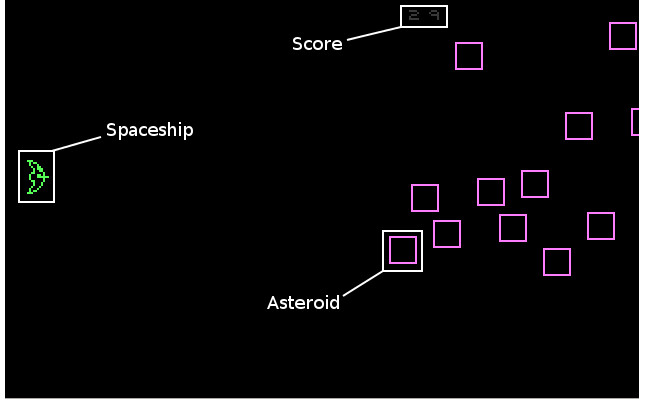
\includegraphics[width=90mm]{In_Game.jpg}
\caption{Wanneer je aan het spelen bent.}
\label{fig:ingame}
\end{figure}

\begin{figure}[htbp]
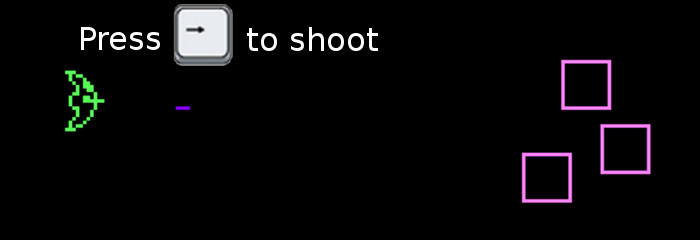
\includegraphics[width=90mm]{PressToShoot.jpg}
\caption{De besturing van het spel}
\label{fig:shoot}
\end{figure}

\begin{figure}[htbp]
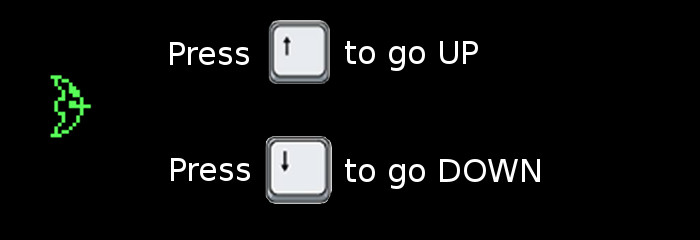
\includegraphics[width=90mm]{Up_Down.jpg}
\caption{De besturing van het spel}
\label{fig:besturing}
\end{figure}

\begin{figure}[htbp]
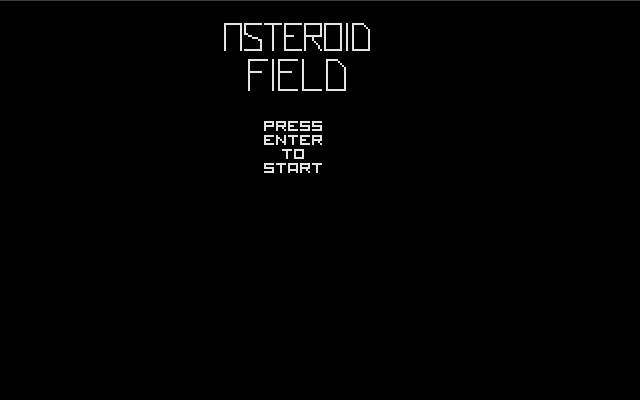
\includegraphics[width=90mm]{Menu.jpg}
\caption{Startscherm}
\label{fig:menu}
\end{figure}

\end{document}
